\documentclass[12pt]{article}
\usepackage{times, latexsym, amsmath, amssymb, amsthm, graphicx, epsfig, fancyhdr}
\usepackage{verbatim}
\usepackage{tikz}
\usepackage{tikz-qtree}
\usetikzlibrary{fit,positioning}
\definecolor{mygray}{RGB}{200,200,200}

\title{HHMM Equations} 
\author {Tim Miller}
%\maketitle

%\setlength{\headheight}{28pt}


\begin{document}
\section{Model equations}
\begin{align*}
p(\vec{s}_t,w_t | \vec{s}_{1,t-1},w_{1,t-1}) &= p(s_t,w_t | s_{t-1}) && \text{Markov Assumption} \\
                                     &= p(s_t|s_{t-1}) p(w_t | s_t) && \text{Word depends only on current state}\\
                                     &= p(f_t,j_t,a_t,b_t,g_t | s_{t-1}) p(w_t | g_t) && \text{s is a joint of multiple sub-variables} \\
                                     &= p_{F}(f_t|s_{t-1}) \cdot \\
                                     &\phantom{{}= } p_{J}(j_t | f_t,s_{t-1}) \cdot\\
                                     &\phantom{{}= } p_{A}(a_t|f_t,j_t,s_{t-1}) \cdot\\
                                     &\phantom{{}= } p_{B}(b_t|c_t,s_{t-1}) \cdot\\
                                     &\phantom{{}= } p_{G}(g_t|c_t,n_t,s_{t-1}) \cdot\\
                                     &\phantom{{}= } p_{W}(w_t|g_t) && \text{Conditional dependencies} 
\end{align*}
                                    

\section{Breakdown of dependencies}
The following covers the $+/+$ case and the $-/-$ case. The other cases are for the first and last word in a sentence and will be handled by special cases for the depth one learner.

\begin{equation}
p_{F}(f_t|s_{t-1}) = p_{FORK}(f_t|b_{t-1},g_{t-1})
\end{equation}

\begin{equation}
p_{J}(j_t|f_t,s_{t-1}) = 
	\begin{cases}
      p_{TRANS}(j_t|b_{t-1},g_{t-1}), & \text{if } f_{t}=+ \\
      p_{RED}(j_t|a_{t-1}), & \text{if } f_{t}=- 
    \end{cases}
\end{equation}

When $f_{t}=+$ the decision of $j$ is whether to TRANSition the awaited category ($j=+$) or create a new stack level. When $f_{t}=-$ the decision of $j$ is whether to REDuce a stack level ($j_t=+$) or replace to do an in-place transition (unary reduction). For the depth one learner this is in fact deterministic since we will know whether we are at the first or last word in the sentence.

\begin{samepage}
\begin{equation}
p_{A}(a_t | s_{t-1},f_t,j_t) = 
  \begin{cases}
   [[a_t==a_{t-1}]], & \text{if } f_{t}=+, j_{t}=+  \\
    p_{ACT}(a_t|a_{t-1}), & \text{if } f_t=-, j_t=- \\
    p_{ROOT}(a_t|a_{t-1},g_{t-1}), &\text{if } f_t=+,j_t=-
  \end{cases}
\end{equation}

Example of $p_{ACT}$: When an NP/NN generates a noun (nn) and is reduced ($f_{t-1}=1$), the next time step might be an S/VP (having completed a noun phrase now we have what might be a sentence lacking only a verb phrase). To generate S we only rely on the previous NP ($a_{t-1}$), given that $f_{t-1}$ was 1.
\end{samepage}

\begin{equation}
p_{B}(b_t | a_t,j_t,f_t,s_{t-1}) = 
  \begin{cases}
   p_{CONT}(b_t|b_{t-1},g_{t-1}), & j_{t}=+ \\
   p_{START}(b_t|a_{t-1},a_t) & j_{t}=-
   \end{cases}
\end{equation}

For the multiple depth learner this will depend on $f_t$ as well but for depth one I believe it only cares about $j_t$ because it will not ever create a new level or collapse a level except deterministically at sentence start and end. So in other words for this model $j_t$ and $f_t$ carry the same information.

Example of $p_{CONT}$: S/VP at $t-1$ generates a verb (V). Then at time $t$ we can't reduce the whole S/VP yet because it requires the rest of the verb phrase. S is copied forward, and the VP ($b_{t-1}$) merges with the V ($g_{t-1}$) to produce an NP at $b_t$ that we would like to see to finish the sentence, and the NP generates a determiner (DT) \emph{the}.

Example of $p_{START}$: NP/NN at $t-1$ generates a common noun ($g_{t-1}$=NN), then $j_t=-$ because the NP is unforked and unjoined ($j_t=-$). $a_t$ transitions to S meaning we now think we are looking for a sentence (S) with the just-completed NP as its subject. $b_{t}$ will be generated using $p_{START}$, using the S from $a_t$ and the NP from $a_{t-1}$ as the conditioning information (representing the rule S $\rightarrow$ NP ?).

\begin{equation}
p_{G}(g_t | s_{t-1},s_t) = p_{POS}(g_t|b_t)
\end{equation}

Part of speech ($g_t$) only depends on the awaited ($b_t$) category at every time step.

\begin{equation}
p_{W}(w_t|s_t) = p_{LEX}(w_t | g_t)
\end{equation}

Lexical item ($w_t$) only depends on the part of speech tag ($g_t$) at the same time step.

\section{Graphical Model}

\begin{figure}[p]
a) F--,J--:\hspace{-15mm}
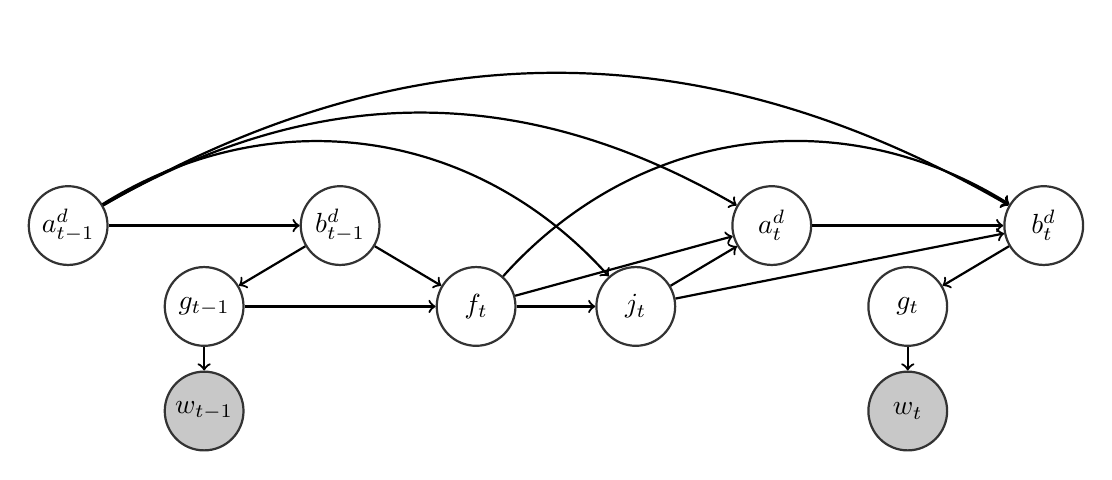
\begin{tikzpicture}[baseline=1cm,node distance=3mm and 10mm,inner sep=0pt]
\tikzstyle{main}=[circle, minimum size = 10mm, thick, draw =black!80]
\tikzstyle{connect}=[-latex, thick,->]
\tikzstyle{from}=[-latex, thick,<-]
\tikzstyle{box}=[rectangle, draw=black!100]
\node[main,fill=white!100] (atp) {$a^d_{t{-}1}$};
\node[main] (gtp) [below right=of atp]{$g_{t{-}1}$};
\node[main] (btp) [above right=of gtp]{$b^d_{t{-}1}$};
\node[main,fill=mygray] (wtp) [below=of gtp]{$w_{t{-}1}$};
\node[main] (ft) [below right=of btp]{$f_t$};
\node[main] (jt) [right=of ft]{$j_t$};
\node[main,fill=white!100] [above right=of jt] (at) {$a^d_t$};
\node[main] (gt) [below right=of at]{$g_t$};
\node[main] (bt) [above right=of gt]{$b^d_t$};
\node[main,fill=mygray] (wt) [below=of gt]{$w_t$};
\path (btp) edge[from] (atp);
\path (gtp) edge[from] (btp);
\path (wtp) edge[from] (gtp);
\path (ft) edge[from] (btp) edge[from] (gtp);
\path (jt) edge[from] (ft) edge[from,bend right=40] (atp);
\path (at) edge[from] (ft) edge[from] (jt) edge[from,bend right] (atp);
\path (bt) edge[from,bend right=40] (ft) edge[from] (jt) edge[from] (at) edge[from,bend right] (atp);
\path (gt) edge[from] (bt);
\path (wt) edge[from] (gt);
\end{tikzpicture}
\vspace{-5mm}

b) F--,J+:\hspace{-15mm}
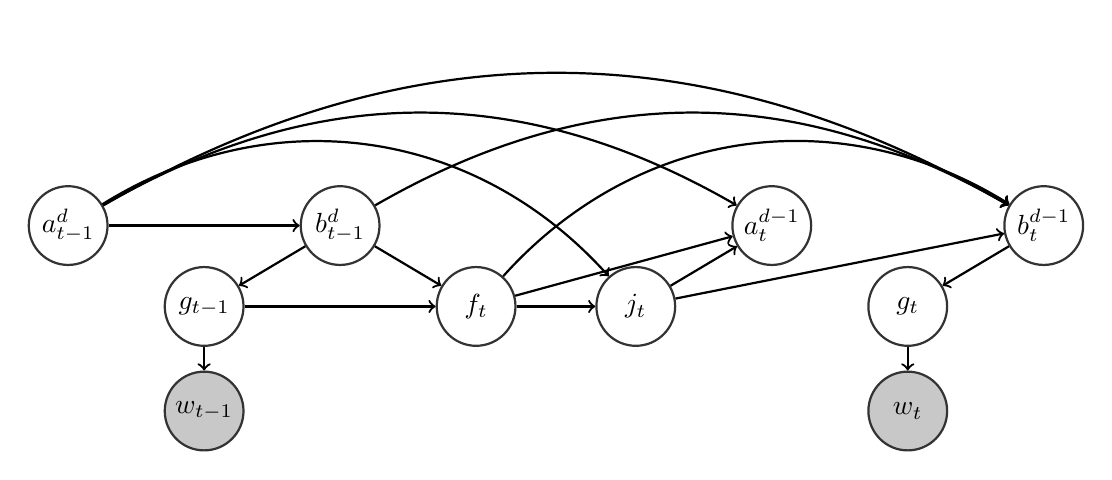
\begin{tikzpicture}[baseline=1cm,node distance=3mm and 10mm,inner sep=0pt]
\tikzstyle{main}=[circle, minimum size = 10mm, thick, draw =black!80]
\tikzstyle{connect}=[-latex, thick,->]
\tikzstyle{from}=[-latex, thick,<-]
\tikzstyle{box}=[rectangle, draw=black!100]
\node[main,fill=white!100] (atp) {$a^d_{t{-}1}$};
\node[main] (gtp) [below right=of atp]{$g_{t{-}1}$};
\node[main] (btp) [above right=of gtp]{$b^d_{t{-}1}$};
\node[main,fill=mygray] (wtp) [below=of gtp]{$w_{t{-}1}$};
\node[main] (ft) [below right=of btp]{$f_t$};
\node[main] (jt) [right=of ft]{$j_t$};
\node[main,fill=white!100] [above right=of jt] (at) {$a^{d{-}1}_t$};
\node[main] (gt) [below right=of at]{$g_t$};
\node[main] (bt) [above right=of gt]{$b^{d{-}1}_t$};
\node[main,fill=mygray] (wt) [below=of gt]{$w_t$};
\path (btp) edge[from] (atp);
\path (gtp) edge[from] (btp);
\path (wtp) edge[from] (gtp);
\path (ft) edge[from] (btp) edge[from] (gtp);
\path (jt) edge[from] (ft) edge[from,bend right=40] (atp);
\path (at) edge[from] (ft) edge[from] (jt) edge[from,bend right] (atp);
\path (bt) edge[from,bend right=40] (ft) edge[from] (jt) edge[from,bend right] (btp) edge[from,bend right] (atp);
\path (gt) edge[from] (bt);
\path (wt) edge[from] (gt);
\end{tikzpicture}
\vspace{-1cm}

c) F+,J--:\hspace{-15mm}
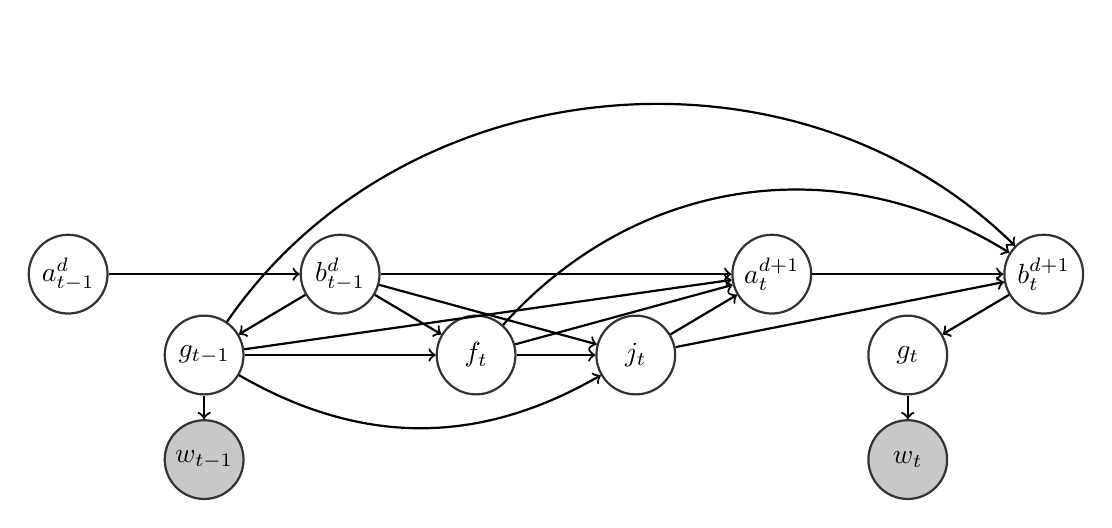
\begin{tikzpicture}[baseline=1cm,node distance=3mm and 10mm,inner sep=0pt]
\tikzstyle{main}=[circle, minimum size = 10mm, thick, draw =black!80]
\tikzstyle{connect}=[-latex, thick,->]
\tikzstyle{from}=[-latex, thick,<-]
\tikzstyle{box}=[rectangle, draw=black!100]
\node[main,fill=white!100] (atp) {$a^d_{t{-}1}$};
\node[main] (gtp) [below right=of atp]{$g_{t{-}1}$};
\node[main] (btp) [above right=of gtp]{$b^d_{t{-}1}$};
\node[main,fill=mygray] (wtp) [below=of gtp]{$w_{t{-}1}$};
\node[main] (ft) [below right=of btp]{$f_t$};
\node[main] (jt) [right=of ft]{$j_t$};
\node[main,fill=white!100] [above right=of jt] (at) {$a^{d{+}1}_t$};
\node[main] (gt) [below right=of at]{$g_t$};
\node[main] (bt) [above right=of gt]{$b^{d{+}1}_t$};
\node[main,fill=mygray] (wt) [below=of gt]{$w_t$};
\path (btp) edge[from] (atp);
\path (gtp) edge[from] (btp);
\path (wtp) edge[from] (gtp);
\path (ft) edge[from] (btp) edge[from] (gtp);
\path (jt) edge[from] (ft) edge[from] (btp) edge[from,bend left] (gtp);
\path (at) edge[from] (ft) edge[from] (jt) edge[from] (btp) edge[from] (gtp);
\path (bt) edge[from,bend right=40] (ft) edge[from] (jt) edge[from] (at) edge[from,bend right=50] (gtp);
\path (gt) edge[from] (bt);
\path (wt) edge[from] (gt);
\end{tikzpicture}
\vspace{-1cm}

d) F+,J+:\hspace{-15mm}
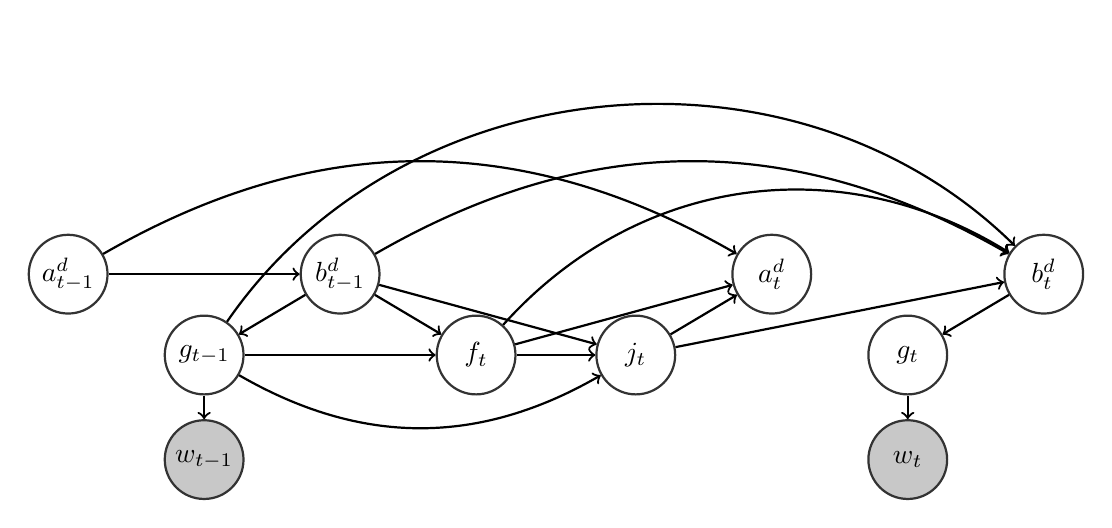
\begin{tikzpicture}[baseline=1cm,node distance=3mm and 10mm,inner sep=0pt]
\tikzstyle{main}=[circle, minimum size = 10mm, thick, draw =black!80]
\tikzstyle{connect}=[-latex, thick,->]
\tikzstyle{from}=[-latex, thick,<-]
\tikzstyle{box}=[rectangle, draw=black!100]
\node[main,fill=white!100] (atp) {$a^d_{t{-}1}$};
\node[main] (gtp) [below right=of atp]{$g_{t{-}1}$};
\node[main] (btp) [above right=of gtp]{$b^d_{t{-}1}$};
\node[main,fill=mygray] (wtp) [below=of gtp]{$w_{t{-}1}$};
\node[main] (ft) [below right=of btp]{$f_t$};
\node[main] (jt) [right=of ft]{$j_t$};
\node[main,fill=white!100] [above right=of jt] (at) {$a^d_t$};
\node[main] (gt) [below right=of at]{$g_t$};
\node[main] (bt) [above right=of gt]{$b^d_t$};
\node[main,fill=mygray] (wt) [below=of gt]{$w_t$};
\path (btp) edge[from] (atp);
\path (gtp) edge[from] (btp);
\path (wtp) edge[from] (gtp);
\path (ft) edge[from] (btp) edge[from] (gtp);
\path (jt) edge[from] (ft) edge[from] (btp) edge[from,bend left] (gtp);
\path (at) edge[from] (ft) edge[from] (jt) edge[from,bend right] (atp);
\path (bt) edge[from,bend right=40] (ft) edge[from] (jt) edge[from,bend right] (btp) edge[from,bend right=50] (gtp);
\path (gt) edge[from] (bt);
\path (wt) edge[from] (gt);
\end{tikzpicture}
\label{fig:hhmm}
\caption{Two time steps of the HHMM model. $s_t$=All hidden variables at time $t$, $a$ = Active category, $b$ = Awaited category, $f$ = Fork node, $j$=Join node $g$ = Part of speech tag, $w$ = word.}
\end{figure}

\begin{figure}[p]
a) F--,J--:\hspace{-15mm}
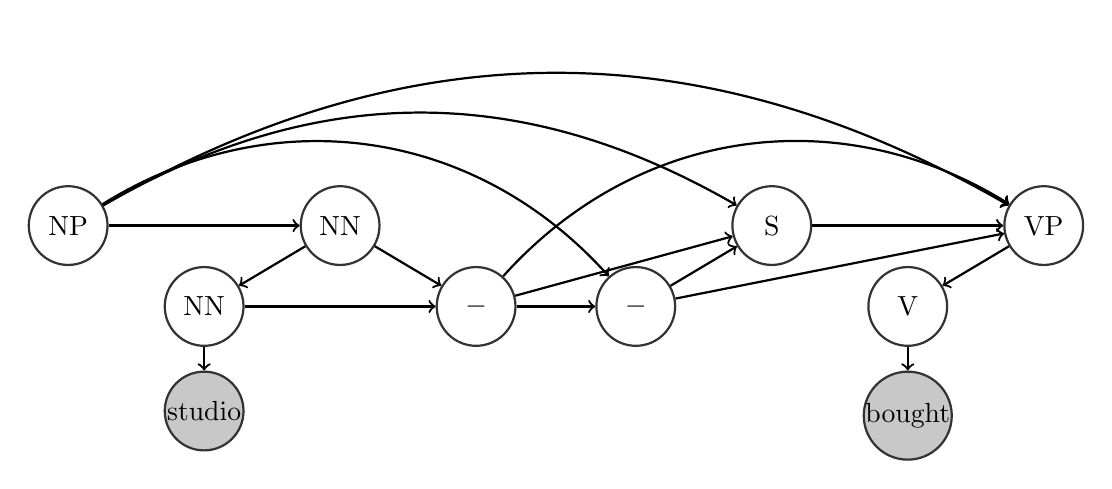
\begin{tikzpicture}[baseline=1cm,node distance=3mm and 10mm,inner sep=0pt]
\tikzstyle{main}=[circle, minimum size = 10mm, thick, draw =black!80]
\tikzstyle{connect}=[-latex, thick,->]
\tikzstyle{from}=[-latex, thick,<-]
\tikzstyle{box}=[rectangle, draw=black!100]
\node[main,fill=white!100] (atp) {NP};
\node[main] (gtp) [below right=of atp]{NN};
\node[main] (btp) [above right=of gtp]{NN};
\node[main,fill=mygray] (wtp) [below=of gtp]{studio};
\node[main] (ft) [below right=of btp]{$-$};
\node[main] (jt) [right=of ft]{$-$};
\node[main,fill=white!100] [above right=of jt] (at) {S};
\node[main] (gt) [below right=of at]{V};
\node[main] (bt) [above right=of gt]{VP};
\node[main,fill=mygray] (wt) [below=of gt]{bought};
\path (btp) edge[from] (atp);
\path (gtp) edge[from] (btp);
\path (wtp) edge[from] (gtp);
\path (ft) edge[from] (btp) edge[from] (gtp);
\path (jt) edge[from] (ft) edge[from,bend right=40] (atp);
\path (at) edge[from] (ft) edge[from] (jt) edge[from,bend right] (atp);
\path (bt) edge[from,bend right=40] (ft) edge[from] (jt) edge[from] (at) edge[from,bend right] (atp);
\path (gt) edge[from] (bt);
\path (wt) edge[from] (gt);
\end{tikzpicture}
\vspace{-5mm}

b) F--,J+:\hspace{-15mm}
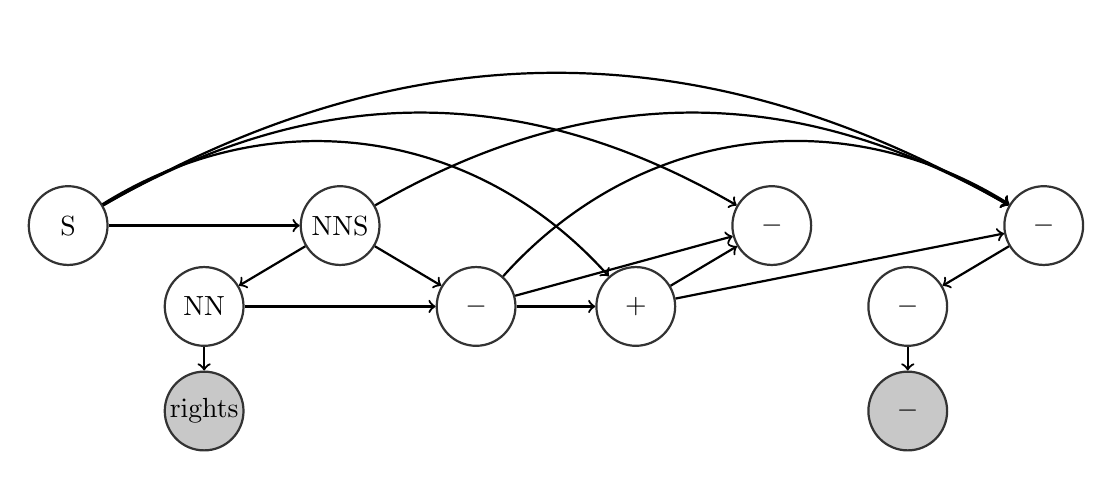
\begin{tikzpicture}[baseline=1cm,node distance=3mm and 10mm,inner sep=0pt]
\tikzstyle{main}=[circle, minimum size = 10mm, thick, draw =black!80]
\tikzstyle{connect}=[-latex, thick,->]
\tikzstyle{from}=[-latex, thick,<-]
\tikzstyle{box}=[rectangle, draw=black!100]
\node[main,fill=white!100] (atp) {S};
\node[main] (gtp) [below right=of atp]{NN};
\node[main] (btp) [above right=of gtp]{NNS};
\node[main,fill=mygray] (wtp) [below=of gtp]{rights};
\node[main] (ft) [below right=of btp]{$-$};
\node[main] (jt) [right=of ft]{$+$};
\node[main,fill=white!100] [above right=of jt] (at) {$-$};
\node[main] (gt) [below right=of at]{$-$};
\node[main] (bt) [above right=of gt]{$-$};
\node[main,fill=mygray] (wt) [below=of gt]{$-$};
\path (btp) edge[from] (atp);
\path (gtp) edge[from] (btp);
\path (wtp) edge[from] (gtp);
\path (ft) edge[from] (btp) edge[from] (gtp);
\path (jt) edge[from] (ft) edge[from,bend right=40] (atp);
\path (at) edge[from] (ft) edge[from] (jt) edge[from,bend right] (atp);
\path (bt) edge[from,bend right=40] (ft) edge[from] (jt) edge[from,bend right] (btp) edge[from,bend right] (atp);
\path (gt) edge[from] (bt);
\path (wt) edge[from] (gt);
\end{tikzpicture}
\vspace{-1cm}

c) F+,J--:\hspace{-15mm}
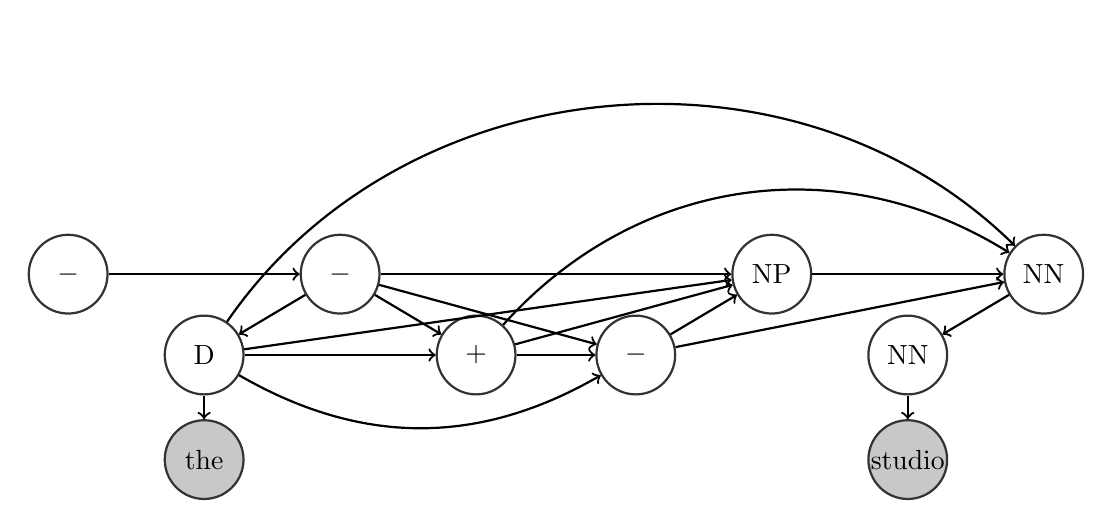
\begin{tikzpicture}[baseline=1cm,node distance=3mm and 10mm,inner sep=0pt]
\tikzstyle{main}=[circle, minimum size = 10mm, thick, draw =black!80]
\tikzstyle{connect}=[-latex, thick,->]
\tikzstyle{from}=[-latex, thick,<-]
\tikzstyle{box}=[rectangle, draw=black!100]
\node[main,fill=white!100] (atp) {$-$};
\node[main] (gtp) [below right=of atp]{D};
\node[main] (btp) [above right=of gtp]{$-$};
\node[main,fill=mygray] (wtp) [below=of gtp]{the};
\node[main] (ft) [below right=of btp]{$+$};
\node[main] (jt) [right=of ft]{$-$};
\node[main,fill=white!100] [above right=of jt] (at) {NP};
\node[main] (gt) [below right=of at]{NN};
\node[main] (bt) [above right=of gt]{NN};
\node[main,fill=mygray] (wt) [below=of gt]{studio};
\path (btp) edge[from] (atp);
\path (gtp) edge[from] (btp);
\path (wtp) edge[from] (gtp);
\path (ft) edge[from] (btp) edge[from] (gtp);
\path (jt) edge[from] (ft) edge[from] (btp) edge[from,bend left] (gtp);
\path (at) edge[from] (ft) edge[from] (jt) edge[from] (btp) edge[from] (gtp);
\path (bt) edge[from,bend right=40] (ft) edge[from] (jt) edge[from] (at) edge[from,bend right=50] (gtp);
\path (gt) edge[from] (bt);
\path (wt) edge[from] (gt);
\end{tikzpicture}
\vspace{-1cm}

d) F+,J+:\hspace{-15mm}
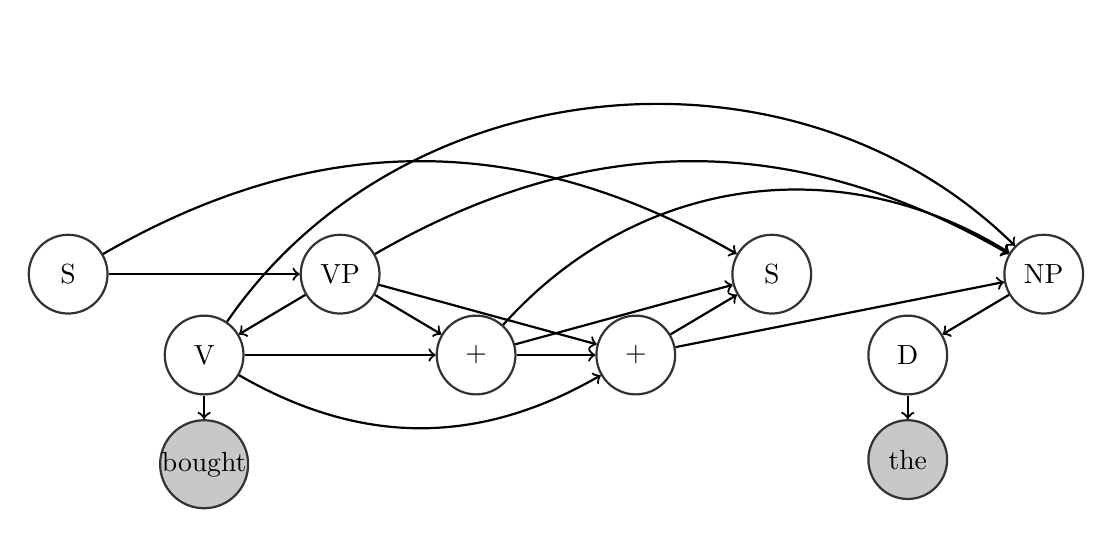
\begin{tikzpicture}[baseline=1cm,node distance=3mm and 10mm,inner sep=0pt]
\tikzstyle{main}=[circle, minimum size = 10mm, thick, draw =black!80]
\tikzstyle{connect}=[-latex, thick,->]
\tikzstyle{from}=[-latex, thick,<-]
\tikzstyle{box}=[rectangle, draw=black!100]
\node[main,fill=white!100] (atp) {S};
\node[main] (gtp) [below right=of atp]{V};
\node[main] (btp) [above right=of gtp]{VP};
\node[main,fill=mygray] (wtp) [below=of gtp]{bought};
\node[main] (ft) [below right=of btp]{$+$};
\node[main] (jt) [right=of ft]{$+$};
\node[main,fill=white!100] [above right=of jt] (at) {S};
\node[main] (gt) [below right=of at]{D};
\node[main] (bt) [above right=of gt]{NP};
\node[main,fill=mygray] (wt) [below=of gt]{the};
\path (btp) edge[from] (atp);
\path (gtp) edge[from] (btp);
\path (wtp) edge[from] (gtp);
\path (ft) edge[from] (btp) edge[from] (gtp);
\path (jt) edge[from] (ft) edge[from] (btp) edge[from,bend left] (gtp);
\path (at) edge[from] (ft) edge[from] (jt) edge[from,bend right] (atp);
\path (bt) edge[from,bend right=40] (ft) edge[from] (jt) edge[from,bend right] (btp) edge[from,bend right=50] (gtp);
\path (gt) edge[from] (bt);
\path (wt) edge[from] (gt);
\end{tikzpicture}
\caption{Same cases as Figure~\ref{fig:hhmm} with concrete examples from the TiCS paper's examples.}
\label{fig:hhmm_eg}
\end{figure}


\def\blue{\color{blue}}
\begin{figure}
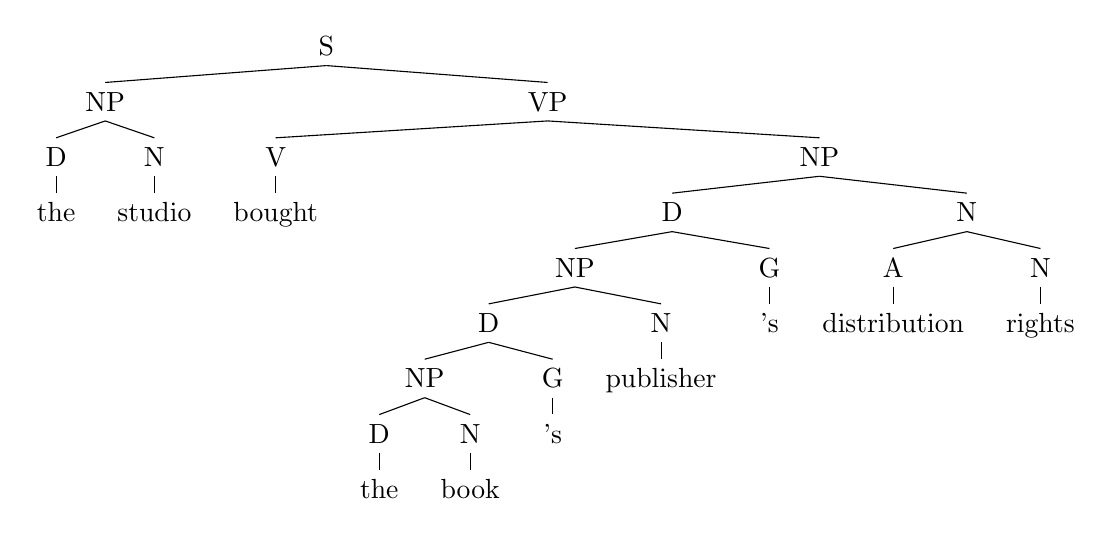
\begin{tikzpicture}[baseline,sibling distance=3mm,level distance=2em]%1.5\baselineskip]
\Tree [.S [.NP [.D {\blue the} ]
               [.N {\blue studio} ] ] 
          [.VP [.V {\blue bought} ]
               [.NP [.D [.NP [.D [.NP [.D {\blue the} ]
                                      [.N {\blue book} ] ]
                                 [.G {\blue 's} ] ]
                             [.N {\blue publisher} ] ]
                        [.G {\blue 's} ] ]
                    [.N [.A {\blue distribution} ]
                        [.N {\blue rights} ] ] ] ] ]
\end{tikzpicture}
\caption{Phrase structure tree for example sentence, `The studio bought the book's publisher's distribution rights.'}
\end{figure}


\begin{comment}

\begin{figure}[p]
\color{red}
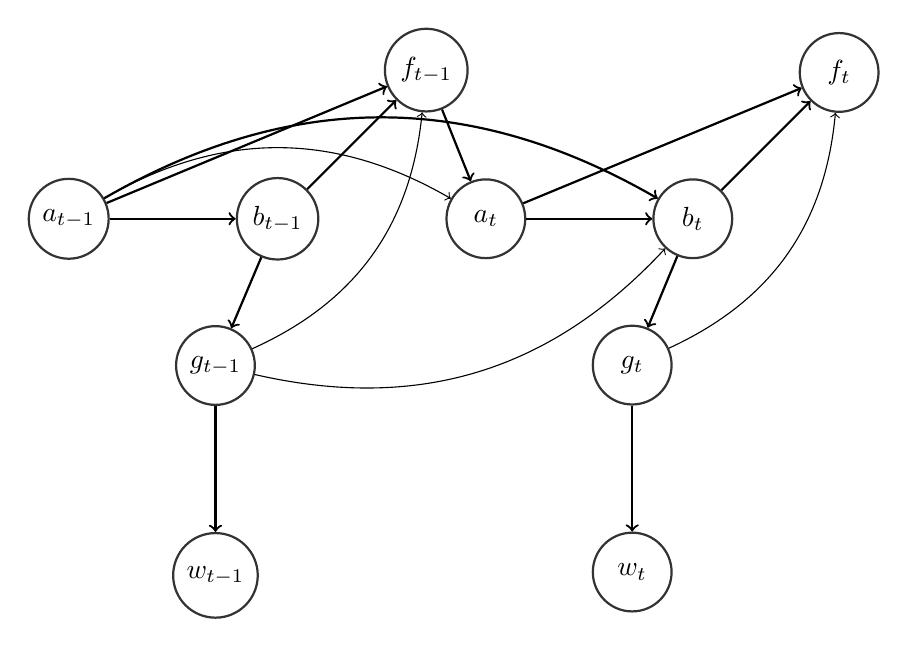
\begin{tikzpicture}
\tikzstyle{main}=[circle, minimum size = 10mm, thick, draw =black!80, node distance = 16mm]
\tikzstyle{connect}=[-latex, thick,->]
\tikzstyle{box}=[rectangle, draw=black!100]
\node[main,fill=white!100] (ctp) {$a_{t-1}$};
\node[main] (ntp) [right=of ctp]{$b_{t-1}$};
\node[main] (gtp) [below right=of ctp]{$g_{t-1}$};
\node[main] (wtp) [below=of gtp]{$w_{t-1}$};
\node[main] (ftp) [above right=of ntp]{$f_{t-1}$};
\node[main,fill=white!100] [right=of ntp] (ct) {$a_t$};
\node[main] (nt) [right=of ct]{$b_t$};
\node[main] (gt) [below right=of ct]{$g_t$};
\node[main] (wt) [below=of gt]{$w_t$};
\node[main] (ft) [above right=of nt]{$f_t$};
\path (ctp) edge [connect] (ntp);
\path (ntp) edge [connect] (gtp);
\path (gtp) edge [connect] (wtp);
\path (ctp) edge [connect] (ftp);
\path (ntp) edge [connect] (ftp);
\path[->] (gtp) edge [bend right] (ftp);
\path[->] (ctp) edge [bend left] (ct);
\path (ftp) edge [connect] (ct);
\path (ctp) edge [connect,bend left] (nt);
\path (ct) edge [connect] (nt);
\path (nt) edge [connect] (gt);
\path (gt) edge [connect] (wt);
\path (ct) edge [connect] (ft);
\path (nt) edge [connect] (ft);
\path[->] (gtp) edge [bend right] (nt);
\path[->] (gt) edge [bend right] (ft);

%  \node[main, fill = white!100] (alpha) [label=below:$\alpha$] { };
%  \node[main] (theta) [right=of alpha,label=below:$\theta$] { };
%  \node[main] (z) [right=of theta,label=below:z] {};
%  \node[main] (beta) [above=of z,label=below:$\beta$] { };
%  \node[main, fill = black!10] (w) [right=of z,label=below:w] { };
%  \path (alpha) edge [connect] (theta)
%        (theta) edge [connect] (z)
%        (z) edge [connect] (w)
%        (beta) edge [connect] (w);
%  \node[rectangle, inner sep=0mm, fit= (z) (w),label=below right:N, xshift=13mm] {};
%  \node[rectangle, inner sep=4.4mm,draw=black!100, fit= (z) (w)] {};
%  \node[rectangle, inner sep=4.6mm, fit= (z) (w),label=below right:M, xshift=12.5mm] {};
%  \node[rectangle, inner sep=9mm, draw=black!100, fit = (theta) (z) (w)] {};
\end{tikzpicture}
\label{fig:hhmmold}
\caption{Two time steps of the HHMM model. $s_t$=All hidden variables at time $t$, $a$ = Active category, $b$ = Awaited category, $f$ = Final node $g$ = Part of speech tag, $w$ = word.}
\end{figure}
\end{comment}


\section{Inference Algorithm}


Randomly initialize all $f, j a, b, g$ for corpus according to constraints (doesn't use models but most be a viable tree). Initialize models ($FORK, TRANS, RED, ACT, CONT, START, POS, LEX$) with counts from random initialization.

\begin{samepage}
\begin{verbatim}
For as long as possible:
  For each sentence:
    Remove all sentence transition counts from model count arrays
    Perform HHMM Forward step from t=1..T:
     f -> j -> a -> b -> g
  
    Sample f,j,a,b,g at time T from subset of states at last time step
  
    Sample backwards through sentence t=T-1..1:
    
      // Jointly sample a,b,g,f
      for (j,f,a,b,g) on beam:
        {j,f,a,b,g}_t ~ p_J(t+1|t) * p_F(t+1|t) *
        			    p_A(t+1|t) * p_B(t+1|t) *
                        p_POS(t+1|t)
      
    Add counts from sentence back to count arrays to make models for
      FORK, TRANS, RED, ACT, CONT, START, POS, LEX
\end{verbatim}
\end{samepage}

\section{Infinite HHMM}

\begin{figure}[t]
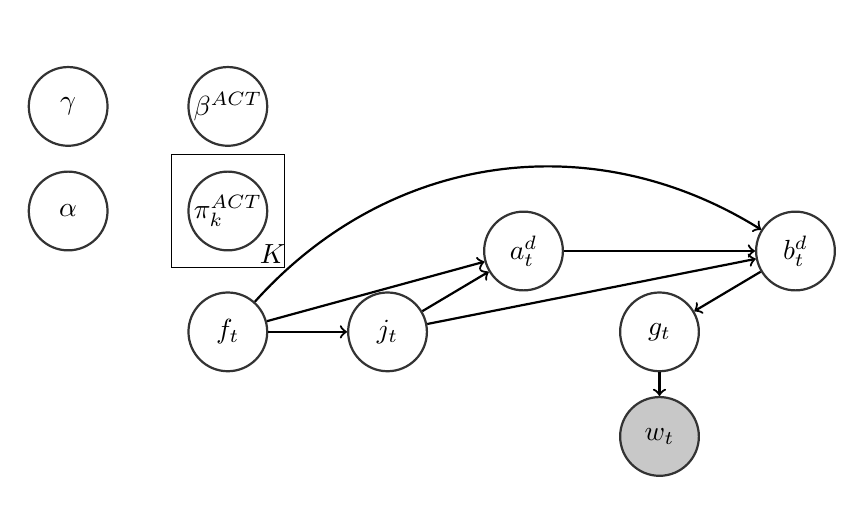
\begin{tikzpicture}[baseline=1cm,node distance=3mm and 10mm,inner sep=0pt]
\tikzstyle{main}=[circle, minimum size = 10mm, thick, draw =black!80]
\tikzstyle{connect}=[-latex, thick,->]
\tikzstyle{from}=[-latex, thick,<-]
\tikzstyle{box}=[rectangle, draw=black!100]
\node[main] (gamma) {$\gamma$};
\node[main] (alpha) [below=of gamma]{$\alpha$};
\node[main] (betaa) [right=of gamma] {$\beta^{ACT}$};
\node[main] (piadp) [below=of betaa] {$\pi_{k}^{ACT}$};
\node[rectangle,inner sep=2mm,draw=black!100,fit= (piadp)] (adp) {};
\node[rectangle,fit=(piadp),label=below right:$K$,xshift=-1.2mm,yshift=1mm]{};

\node[main] (ft) [below=of adp]{$f_t$};
\node[main] (jt) [right=of ft]{$j_t$};
\node[main,fill=white!100] [above right=of jt] (at) {$a^d_t$};
\node[main] (gt) [below right=of at]{$g_t$};
\node[main] (bt) [above right=of gt]{$b^d_t$};
\node[main,fill=mygray] (wt) [below=of gt]{$w_t$};
\path (jt) edge[from] (ft);
\path (at) edge[from] (ft) edge[from] (jt);
\path (bt) edge[from,bend right=40] (ft) edge[from] (jt) edge[from] (at) ;
\path (gt) edge[from] (bt);
\path (wt) edge[from] (gt);
\end{tikzpicture}

\end{figure}

















\end{document}